% Appendix Template

\chapter{WT\_Perf} % Main appendix title

\label{AppendixE} % Change X to a consecutive letter; for referencing this appendix elsewhere, use \ref{AppendixX}

\lhead{Appendix E. \emph{WT\_Perf}} % Change X to a consecutive letter; this is for the header on each page - perhaps a shortened title

WT\_Perf uses blade-element momentum (BEM) theory to predict the aerodynamic performance of a turbine rotor for a given set of operating conditions. WT\_Perf was written by National Wind Technology Center (NWTC) staff at the National Renewable Energy Laboratory (NREL) and is descended from the PROP simulation tool developed at Oregon State University. WT\_Perf is documented in \cite{buhl2012} and \cite{buhl2012}. However, NREL has stopped supporting WT\_Perf since the work in Chapter \ref{Chapter2} was performed and \cite{buhl2012} is no longer readily available.

The aerodynamics of a wind turbine rotor are complex and three dimensional. For a typical wind turbine blade the chord length, twist angle, and airfoil shape change along the length of the blade. In addition, the blade follows a circular trajectory so the end of the blade does not see the same apparent wind as the base of the blade. Simulating the entire rotor would be difficult and computationally expensive. However, a more computationally efficient estimate of rotor performance can be obtained by breaking this large complex 3-D problem into many smaller 2-D simulations. In essence, blade-element momentum theory (BEM) models each wind turbine blade as a collection of many blade elements of width $\delta{r}$ subject to 2-D airflow (Figure \ref{figE-1}). If $\delta{r}$ is small enough the chord length, twist angle, airfoil shape, and apparent wind can be considered constant along the width of each blade element. The aerodynamic forces on the rotor can then be determined by summing the forces on all of the blade elements and applying a series of correction factors to account for 3-D flow effects such as tip vortices, root vortices, and dynamic stall. 



\begin{figure}[ht]
	\centering
		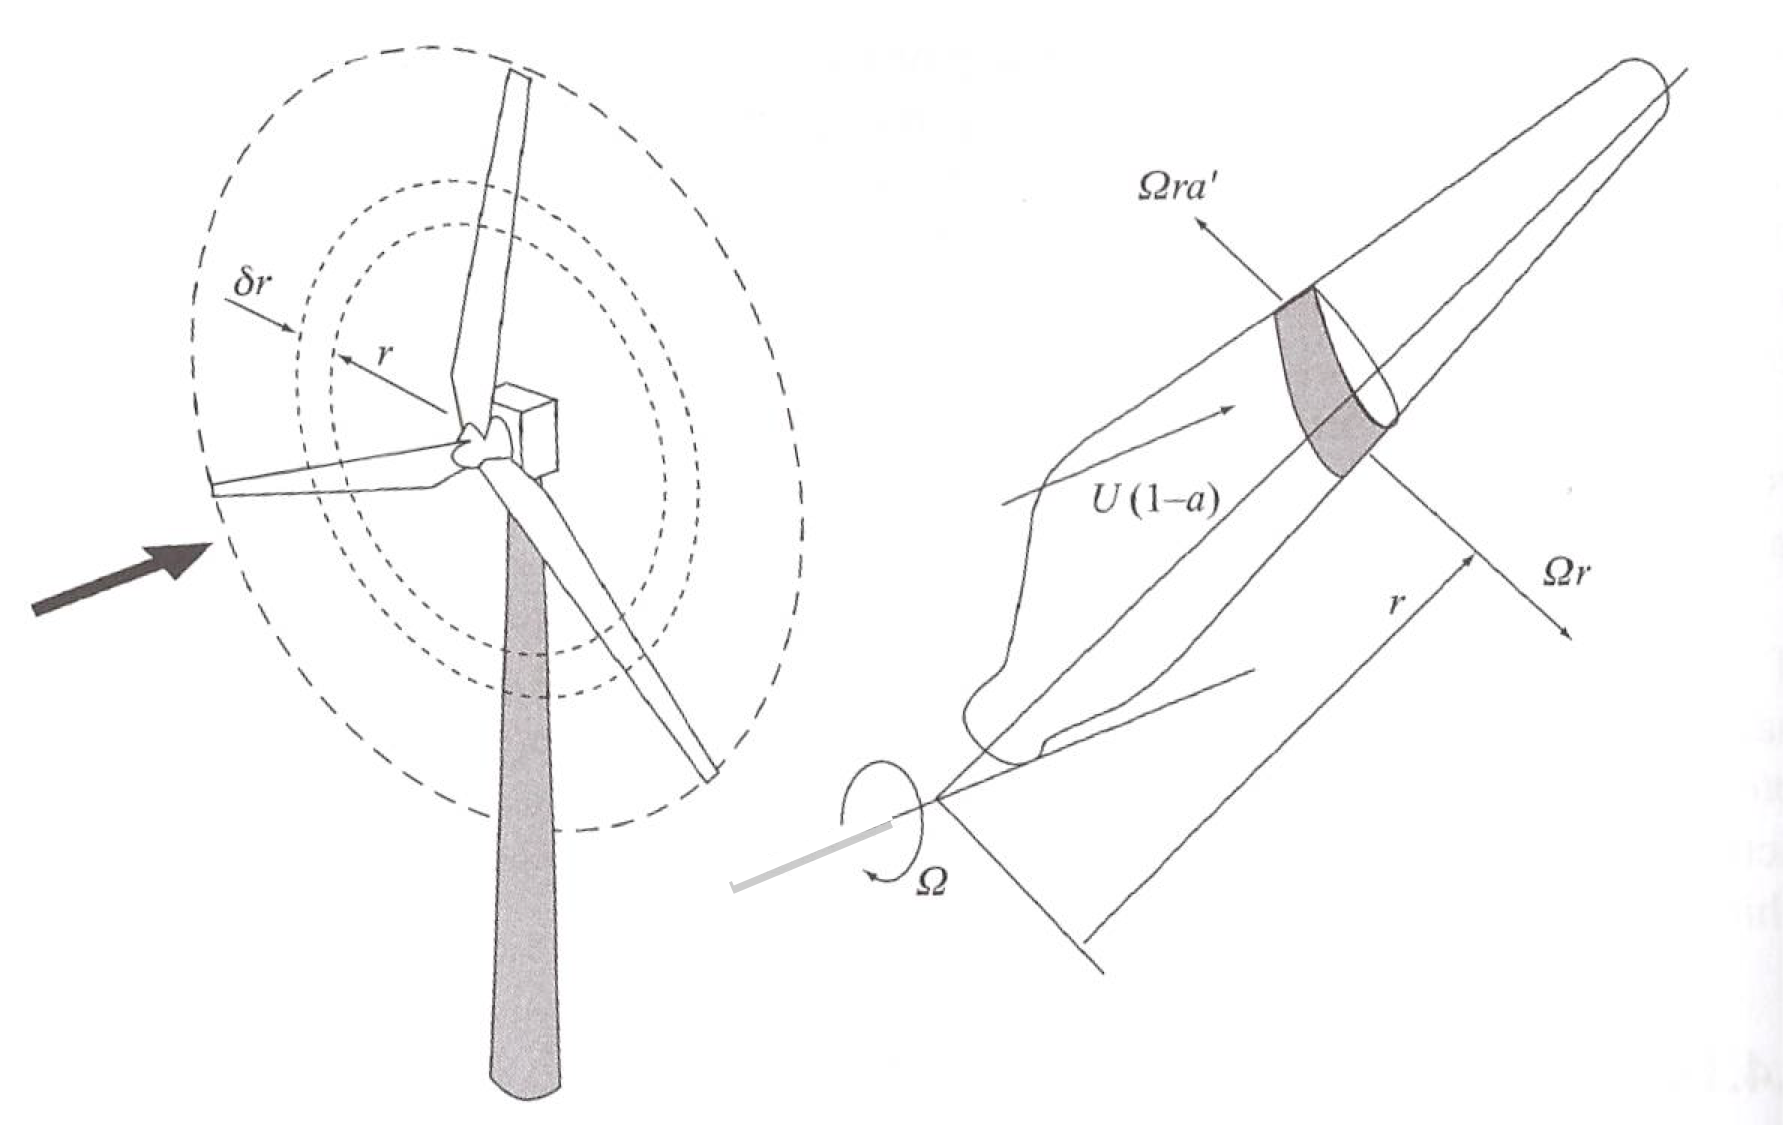
\includegraphics[width=.75\textwidth]{Figures/AppendixEFigures/figE-1.png}
	\caption{BEM models each turbine blade as a collection of spanwise blade segments.\cite{burton2011}}
	\label{figE-1}
\end{figure}


Section \ref{sectionE-1} contains a typical WT\_Perf input file. The \textit{Model Configuration} and \textit{Algorithm Configuration} sections define the BEM methods to be used. \textit{Model Configuration} specifies how many elements each blade will be divided into (Numsect) and specifies the tolerances used to determine adequate convergence of the iterative BEM calculations. \textit{Algorithm Configuration} controls a set of optional correction factors that can be applied to BEM calculations. Some of these correction factors (such as TipLoss, HubLoss, and Swirl) approximate 3-D flow effects that would not otherwise be captured by BEM. The \textit{Turbine Data} and \textit{Aerodynamic Data} sections define the turbine rotor being modeled. \textit{Turbine Data} quantifies many physical properties of the rotor, including the number of blades (NumBlade) as well as the physical dimensions, location, and orientation of the rotor (RotorRad, HubRad, PreCone, Tilt, Yaw, HubHt). The remainder of \textit{Turbine Data} defines each turbine blade by describing a series of blade segments. Each segment has a defined radial length (RElm), axial twist (Twist), chord length (Chord), and airfoil shape (AFfile). \textit{Aerodynamic Data} contains information required for aerodynamic calculations. The first three lines (Rho, KinVisc, and Shear) contain physical properties of the incoming wind. The remainder of \textit{Aerodynamic Data} defines a set of \textit{.dat} files that contain detailed descriptions of airfoil shapes that make up the turbine blade. 

Unlike FAST, which is discussed in Appendix \ref{AppendixA}, WT\_Perf cannot model turbine controls and cannot model dynamic turbine behavior, such as the effect of changing wind speed, changing rotor speed, or changing blade pitch. However, for a given set of operating conditions (blade pitch, rotor speed, and wind speed) WT\_Perf can calculate the rotor power, power coefficient ($C_p$), shaft torque, flap bending moment, and/or rotor thrust. Calculating rotor performance based on specified operating conditions instead of dynamic turbine behavior makes WT\_Perf very computationally inexpensive. WT\_Perf can calculate rotor performance metrics for thousands of operating conditions in a few minutes.  

The \textit{Combined-Case Analysis} and \textit{Parametric Analysis} sections of the WT\_Perf input file tell WT\_Perf which rotor performance metrics to output and which operating conditions to perform BEM calculations for. The input file shown below instructs WT\_Perf to calculate the power coefficient ($C_p$) for all integer blade pitches between -5\degree\ and 5\degree\, all integer rotor speeds between 1 RPM and 14 RPM, and all integer wind speeds between 3 m/s and 16 m/s. This causes WT\_Perf to calculate $C_p$ at 2,156 sets of operating conditions (11 blade pitches $\times$ 14 rotor speeds $\times$ 14 wind speeds). In this dissertation, parametric analyses like the one corresponding to this input file were used to characterize the relationship between $C_p$, tip speed ratio ($\lambda$), and blade pitch for the NREL 5-MW turbine. The relationship between those parameters is illustrated in Figures \ref{fig2-13} and \ref{fig2-14} and enables wind speed estimation based on rotor dynamics (as described in Section \ref{section2-4}).

\pagebreak
\section{Example WT\_Perf input file.} \label{sectionE-1}

\noindent
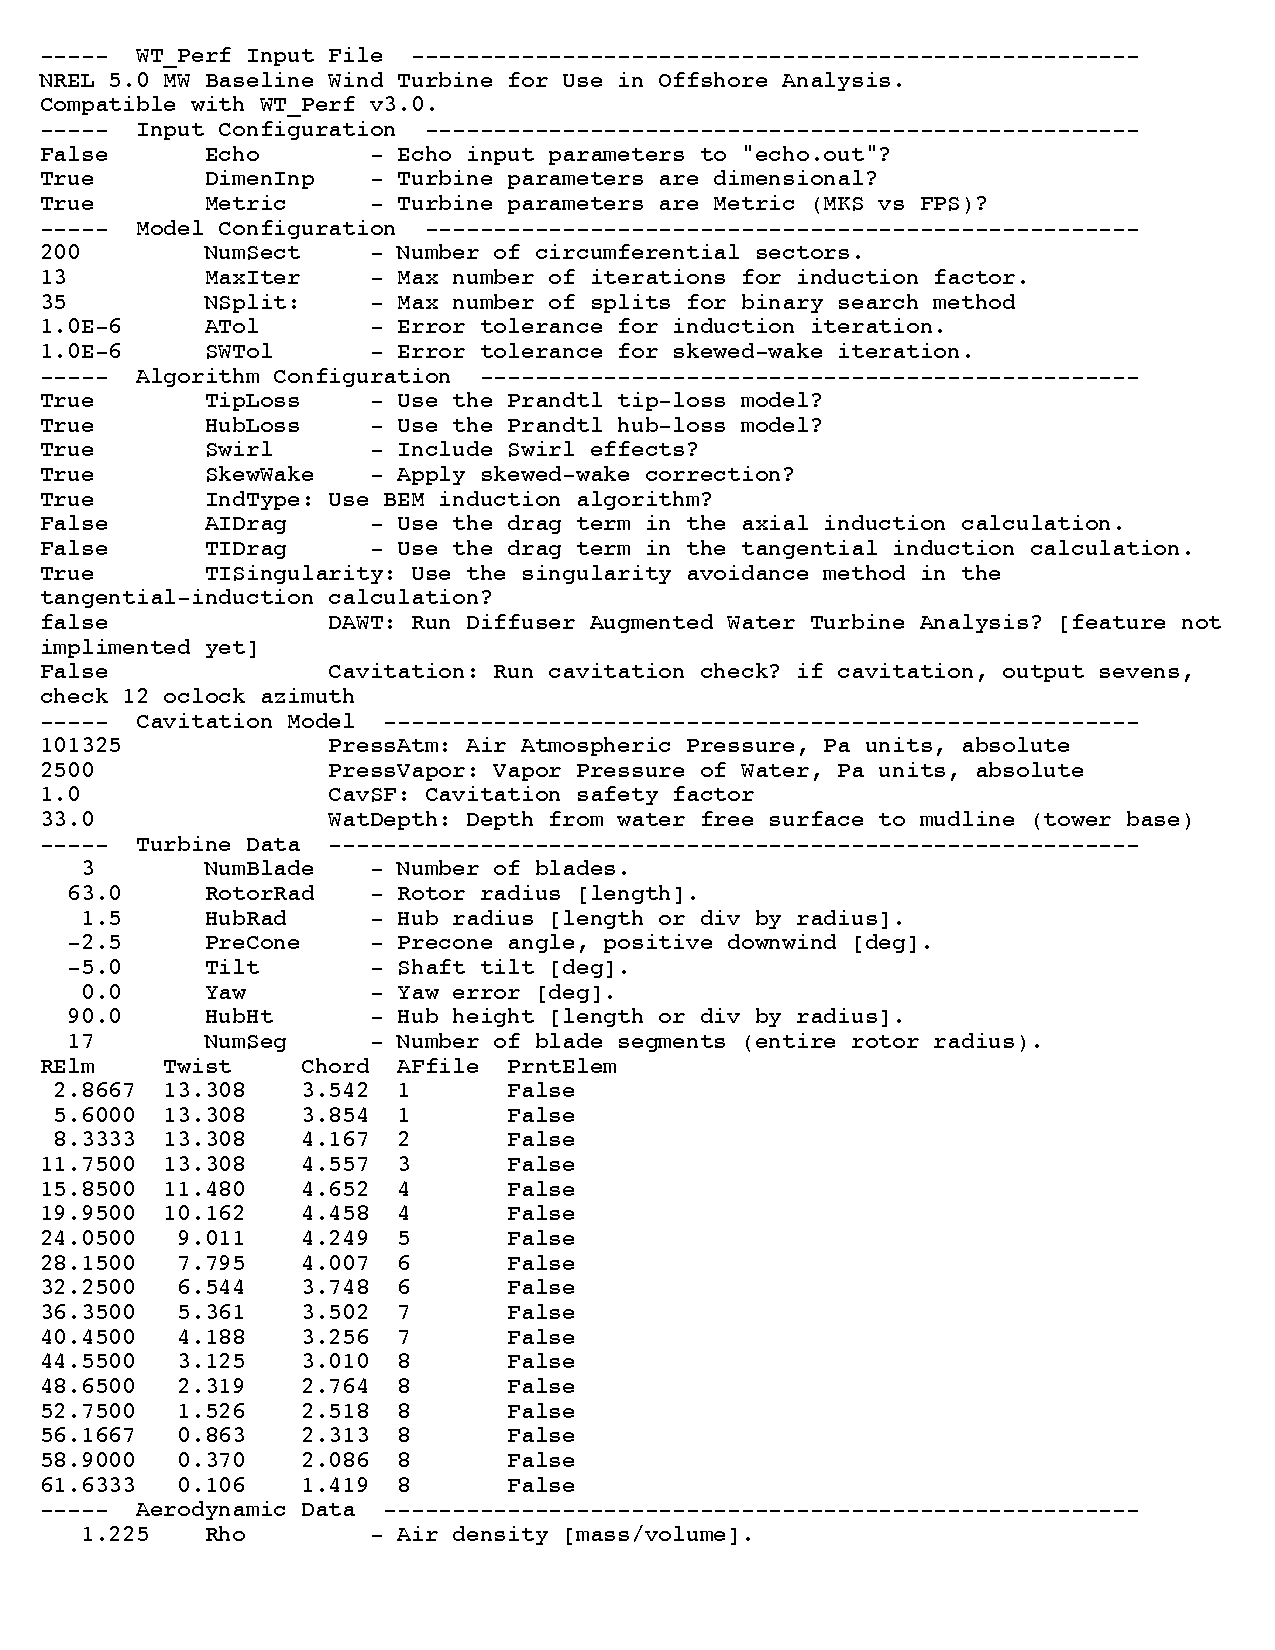
\includegraphics[width=\linewidth]{Figures/AppendixEFigures/figE-2.pdf}	

\noindent
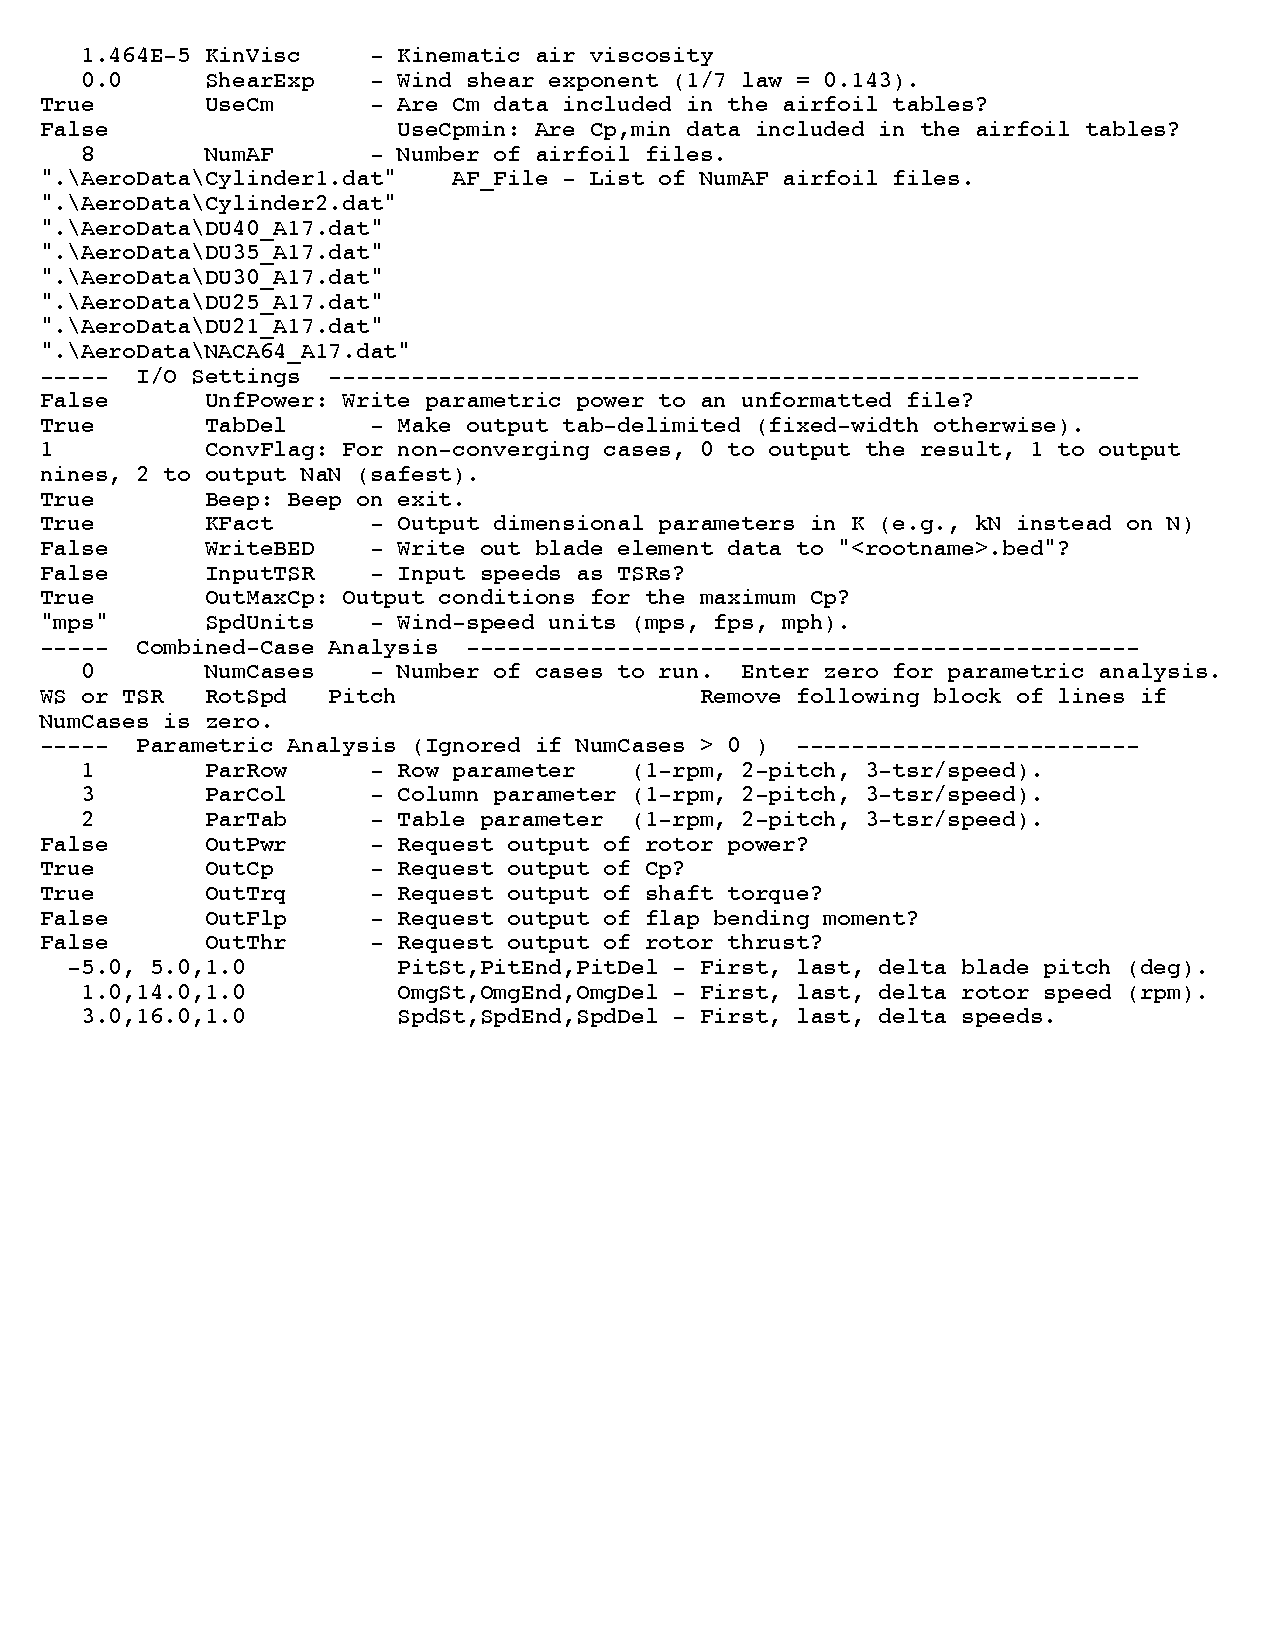
\includegraphics[width=\linewidth]{Figures/AppendixEFigures/figE-3.pdf}